
% this file is called up by thesis.tex
% content in this file will be fed into the main document

%: ----------------------- introduction file header -----------------------
\chapter{Introduction and related work}

% the code below specifies where the figures are stored
\graphicspath{{1_introduction/}}

\begin{abstract}{Résumé}

\end{abstract}

\begin{abstract}{Abstract}

We aim in this chapter at providing some background on biological and
mathematical concepts present in this thesis.

\end{abstract}


\section{Peeking under the hood of genome architecture}

Methods to investigate the 3D structure of the genome fall broadly into two
categories: bio imaging techniques and biochemical protocols. In the first
category, light microscopy allows single cell visualization of specific loci
and enables live cell imaging, sometimes at very high resoluton
\citep{cremer:chromosome-2010}. Yet, these techniques limit studies to a very
small number of loci. On the other hand, biochemical protocols, such as
chromosome conformation capture (3C) and its derivatives, enable to measure
physical interaction between DNA fragments \cite{dekker:capturing}, but
performing single cell experiments is troublesome, and tracking live cell
impossible. In this thesis, we are mostly interested in analysing 3C and such
datasets.

\subsection{3C, 4C, 5C and Hi-C data}

 In recent years, the technique of chromosome conformation capture (3C)
\citep{dekker:capturing}, which identifies physical contacts between different
genomic loci and yields information about their relative spatial distance in
the nucleus, has paved the way for the systematic analysis of the 3D structure
of DNA. 3C techniques and its derivatives are based on 5 experimental steps
\citep{lieberman-aiden:comprehensive, kalhor:genome}.

\begin{itemize}
\item \textbf{Cross-linking} : results in the cross-linking of DNA segments to
proteins and to cross-linking of proteins with each other.
\item \textbf{Restriction digest} A restriction enzyme is added in excess to
the cross-linked DNA. The restriction enzyme will cut the DNA at specific
nucleotide sequences, separating the non-cross-linked DNA from the
cross-linked chromatin. Recognition sequences in DNA differ from each
restriction enzyme, producing different lengths and sequences of strands.
The selection of the restriction enzyme depends on the type of studies
targeted in the experiment.
\item \textbf{Intramolecular Ligation} The third step is an intramolecular
ligation step. DNA fragments are binded together. There are two major types
of ligation junctions: the first is the ligation of two neighboring DNA
fragments, and the second is the junction that is formed when ligating one end
of the fragment to the other end of the same fragment. The latter represents
around 30\% of the junctions formed.
\item \textbf{Reverse Cross-links} The fourth step consists of reversing the
first step: the reversal of cross-links.
\item \textbf{Quantitation} Polymerase chain reaction (PCR) is used to amplify
the DNA copies and to assess the frequencies of the fragments of interest,
which are then sequenced.
\end{itemize}

\begin{figure}
\begin{center}

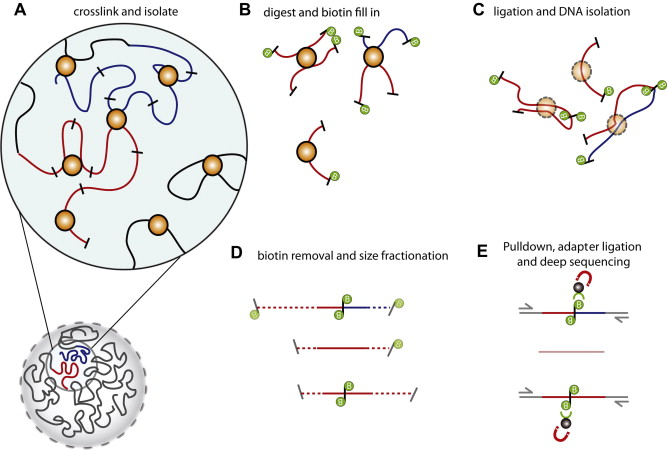
\includegraphics[width=0.8\linewidth]{figures/hic_protocol.png}
\end{center}
\caption{\textbf{Hi-C Protocol.} The procedure relies on cross linking,
restriction enzymes digestions, intra molecular ligation, deproteinization and
deep sequencing. Reads are then aligned to the reference genome, and binned at
$10kb$, $40bk$ or $100kb$ depending on coverage.}
\end{figure}


After paired-end sequencing, each pair of reads can be associated to one
\citep{lieberman-aiden:comprehensive} or several \citep{ay:identifying} DNA
interactions. We can then create a symmetric hollow matrix of integers, for
which entries correspond to the number of reads that fall into a bin. We
denote by $C$ the interaction frequency matrix, and $c_{ij}$ the interaction
frequency between locus $i$ and locus $j$.

These protocols are complex, and yield highly biased interaction frequencies
\citep{imakaev:iterative, cournac:normalization, yaffe:probabilistic}.
\citet{imakaev:iterative} proposes a simple iterative method, called ICE, to
normalize the data. In short, the authors assume that the bias of each entry
$c_{ij}$ of the matrix can be written as the product of two biases $\beta_i$
and $\beta_j$ corresponding to biases induced by loci. Hence, we can write
$c_{ij} = \beta_i \beta_j p_{ij}$, where $p_{ij}$ is the probability of locus
$i$ interacting with locus $j$. Thus, $\sum_i p_{ij} = 1$. This is a non convex
optimization problem that can be solved exactly by an iterative process. To
avoid degeneracies, we filter out the top 2\% sparse loci from our entry
matrix before applying ICE. To give an intuition, this method projects each
vector of interactions onto the $\ell_1$ unit ball. In practice, it yields an
expected interaction frequency count: $k p_{ij}$, where $k$ is the mean
interaction frequency.

Thought still quite recent, chromosome conformation capture and its genome
wide derivatives are now widely used to discover how DNA folds in a bunch of
different organisms \citep{duan:three, sexton:three-dimensional,
tanizawa:mapping, ay:three-dimensional}. The challenge is now to increase the
Hi-C resolution, using very large data sets with deeper sequencing
\citep{rao:3d, jin:high-resolution}. As any genome-wide sequencing data, Hi-C
usually requires several millions or billions of paired-end sequencing reads,
depending on genome size and on the desired resolution. Managing these data
thus requires optimized bioinformatics workflows able to extract the contact
frequencies in reasonable computational time and with reasonable storage
requirements. The overall strategy to analyze Hi-C data is converging among
recent studies and summarized in \cite{lajoie:hitchhiker}. Our collaborators
and we have built HiC-Pro, an an easy-to-use and complete pipeline to process
Hi-C data from raw sequencing reads to the normalized contact maps.

\section{The study of chromosome organization}

The study of chromosome organization broadly falls into two categories:
model-based studies and data-driven studies. The former methods consider the
polymer nature of DNA to leverage the theoretical and computational work done
statistical physics of polymers, to built, with as few assumptions as
possiblemany possible chromosome conformations. Those chromosome conformations
are then used to compare against experimental data, such as Hi-C contact
counts matrices, in order to iteratively improve the models. These models
offer mechanistical insights into the folding of DNA. The latter approaches
use the experimental data to infer 3D models, by typically minizing a cost
function ensuring the models are as consistent as possible with the data.

We will review some techniques develpped to study the folding of DNA, mostly
data-driven models. \citet{rosa:computational} provide a more more complete
overview of computational models of genome architectures.

Several techniques have been developed to infer three-dimensional models of
the genome from interaction counts data. They fall into three categories: the
first finds an average structure by optimizing an objective function as
\citep{tanizawa:mapping, duan:three, ben-elazar:spatial}. The
second samples local minima from a optimization problem leading to the study
of the population of local minima \citep{bau:three-dimensional}. The last
samples the posterior distribution \citep{rousseau:three}.

\citet{tanizawa:mapping} model the 3D genome of the fission yeast (3
chromosomes) by a string of $622$ beads, each bead $x_i$ being the center of a
$20$kb section. The first step was to infer physical distances $\delta_{ij}$
from frequency interactions. They studied eighteen pairs of genes using FISH
measurements, and fitted the Hi-C data on the distances with a non linear
regression curve. The second step was to compute the coordinates of the beads,
such that the distances between the beads matches the inferred physical
distances to the best, with additional biological motivated constraints.

\citet{duan:three} converts the interaction frequencies into distances by
examining the relationship between interaction frequencies and genomic
distances. Then, a multidimensional scaling (MDS) is used to place each bead
so that the wish distances are respected as well as possible.

\citet{tanizawa:mapping} and \citet{duan:three} optimizes a problem of the
form:
\begin{equation*}
\renewcommand{\arraystretch}{2}
\begin{array}{ccll}
\underset{x_1,\ldots, x_n}{\text{minimize}} & & 
\underset{i<j\leq n}{\sum} \big(\|x_i - x_j\|_2 - \delta_{ij}\big)^2 &\\
\text{subject to}
& & \text{biological motivated non convex constraints.}
\end{array}
\end{equation*}

\citet{tanizawa:mapping} published one solution, but did not mention the non
convexity of the problem. Hence, we assume they seeked the best local minimum
\citet{duan:three} ran the optimization process 30 times, and, observing the
obtained solutions, found that they did not differ much. No formal study was
done to compare the solutions.

\citet{ben-elazar:spatial} formulated a non metric multidimensional scaling
optimization problem. They first filtered the interaction count matrix so that
remained only the most significant interactions. They then interpolated the
missing values to obtain a smooth, symmetric, positive definite matrix.

\citet{bau:three-dimensional} used IMP (Integrative Modeling Platform), also
used in nuclear magnetic resonance (NMR) microscopy to construct a 3D model of
the $\alpha$-globin module. Chromosomes are represented by beads, each beads
linked by restraining oscillators. IMP seeks a solution at the equilibrium of
those beads. Three types of restraints are used: the first  corresponds to
harmonic oscillators, with strengths inversely proportional to the 5C
score, computed from the interaction frequencies. The second ensures that two
beads cannot be too close to each other. The third ensure that two consecutive
beads cannot be separated too much. The last two springs have strength only
when the constraints are not fulfilled. The optimization of this problem
yields different configuration with similar IMP scores. A population of 50000
structures was computed. The 10000 structures with the smaller objective
function were then chosen as the population of local minima to be studied.

\citet{rousseau:three} describes a formal probabilistic model of interaction
frequencies and their relationship with physical distances by hypothesizing
that interaction frequencies are inversely proportional to distances. They
then use a Markov Chain Monte Carlo sampling procedure on an optimization
problem that uses the same objective function as \citet{tanizawa:mapping} and
\citet{duan:three} to produce an ensemble of 3D structures.

Finally, \citet{tjong:physical} constructs a very simple model by
modeling chromosomes as a flexible fiber, and using additional biologically
motivated constraints, such as the positioning of centromeres and telomeres,
they formulate an optimization problem. Generating $200000$ feasible
structures, they show that Hi-C data can be fully explained by this very
simple model.

\begin{table}[ht!]
\caption{\bf A comparison of 3D inference methods}
\begin{center}
\begin{tabular}{lrcrr}
\hline
\emph{Publication} & \emph{Name} & \emph{Cons or Pop} & \emph{MDS-based} & Available \\
\hline
\citet{duan:three} & - & Cons & & Y \\
\citet{tanizawa:mapping} & & Cons & & N \\
\citet{ay:three-dimensional} & & Cons & & N\\
Nature methods & & Cons & & N\\
\citet{ben-elazar:spatial} & & Y & & N \\
\citet{varoquaux:statistical} & Y & N & & Y\\
\citet{bau:three-dimensional} & & & &\\
\citet{umbarger:three-dimensional} & & & &\\
\citet{zhang:inference} & chromSDE & & &\\
\citet{rousseau:three} & & & &\\
\citet{hu:bayesian} & & & &\\
\citet{kalhor:genome} & & & &\\
\citet{tokuda:dynamical} & & & &\\
\citet{wong:predictive} & & & &\\
\citet{gehlen:chromosome} & & & &\\
Alber & & & &\\
\end{tabular}
\end{center}
\end{table}


\section{Long range interactions}


Contact counts maps have recently been re-purposed for diverse applications,
far outside the study of the conformation of chromosomes: \textit{de novo}
genome assembly \citep{burton:chromosome, kaplan:high-throughput},
deconvolution of metagenomic samples \citep{burton:species-level,
beitel:strain}, and genome annotation \citep{marie-nelly:filling,
varoquaux:accurate}. Indeed, these maps contain long range contiguity
information that can be used in a wide range of applications.
In this section, we review the applications and methods used.


\section{Contributions}

